% !TEX TS-program = pdflatex
% !TEX encoding = UTF-8 Unicode

\documentclass{beamer}
% for handouts: \documentclass[handout]{beamer}

%\setbeamertemplate{background canvas}[vertical shading][bottom=white,top=structure.fg!25]
% or whatever

\usetheme[compress]{Amsterdam}
%\setbeamertemplate{headline}{}
%\setbeamertemplate{footline}{}
%\setbeamersize{text margin left=0.5cm}
  
\usepackage[english]{babel}
\usepackage{listings}
\usepackage{geometry}
\usepackage{hyperref}
\usepackage{multicol}



\usepackage{color}

\usepackage[utf8]{inputenc}
\usepackage[T1]{fontenc}
\usepackage{lmodern}

\lstset{
basicstyle=\scriptsize\ttfamily,
columns=flexible,
breaklines=true,
numbers=left,
%stepsize=1,
numberstyle=\tiny,
backgroundcolor=\color[rgb]{0.85,0.90,1}
}


\begin{document}

\title{Working with text: Topic modelling}
\author[Damian Trilling]{Damian Trilling \\ ~ \\ \footnotesize{d.c.trilling@uva.nl \\@damian0604} \\ \url{www.damiantrilling.net}}
\date{18--1--2018}
\institute[UvA]{Afdeling Communicatiewetenschap \\Universiteit van Amsterdam}



\begin{frame}{}
\titlepage
\end{frame}

\begin{frame}{Today}
\tableofcontents
\end{frame}



\section[Automated Content Analysis]{Automated Content Analysis (ACA)}
\begin{frame}[plain]
	What's Automated Content Analysis?
\end{frame}


\begin{frame}[plain]
\begin{figure}
\centering
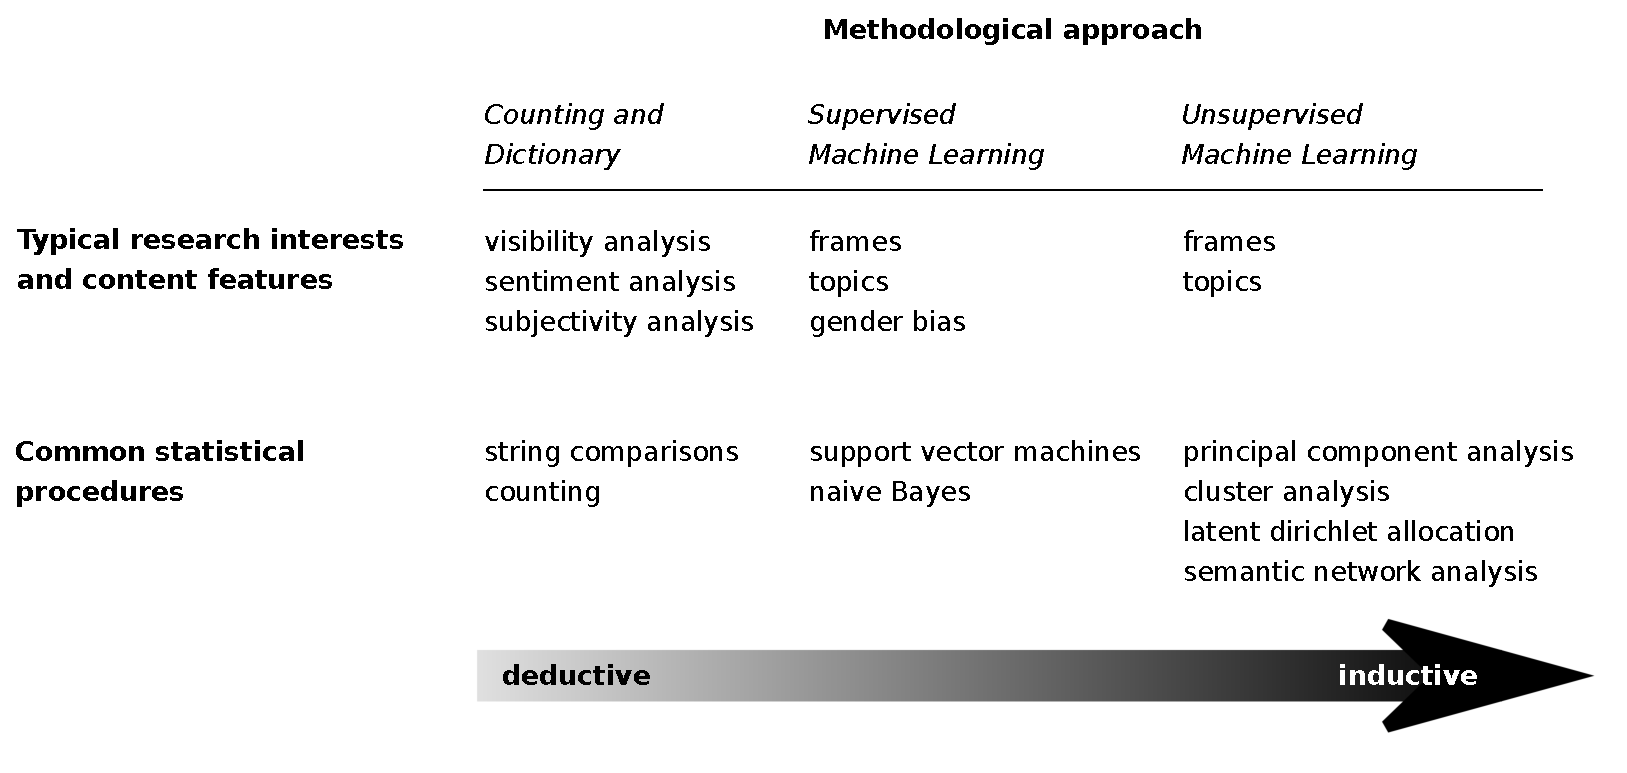
\includegraphics[width=1.0\linewidth]{boumanstrilling2016}
\label{fig:boumanstrilling2016}
\end{figure}
\tiny{Boumans, J. W., \& Trilling, D. (2016). Taking stock of the toolkit: An overview of relevant autmated content analysis approaches and techniques for digital journalism scholars. \emph{Digital Journalism, 4}(1), 8–23. doi:10.1080/21670811.2015.1096598}
\end{frame}




\section[Basic ACA]{Basic top-down ACA: Dictionary- and string-based methods}

\subsection{Regular expressions}
\begin{frame}
	\textbf{Basic ACA: Dictionary- and string-based methods}\\
	Regular expressions
\end{frame}


\begin{frame}{Regular Expressions: What and why?}
\begin{block}{What is a regexp?}
\begin{itemize}
\item<1-> a \emph{very} widespread way to describe patterns in strings
\item<2-> Think of wildcards like {\tt{*}} or operators like {\tt{OR}}, {\tt{AND}} or {\tt{NOT}} in search strings: a regexp does the same, but is \emph{much} more powerful
\item<3-> You can use them in many text editors (!), in STATA, R, Python, \ldots 
\end{itemize}
\end{block}
\end{frame}

\begin{frame}{An example}
\begin{block}{We wanted to find references to companies in several years of news coverage}
Problems: 
\begin{itemize}
\item Spelling variations (ABN, ABN Amro, ABN-Amro, \ldots)
\item Shouldn't be in the middle of the word, but \emph{can} be at the beginning of a word, optionally connected with a hyphen (``ABN-topman'', ``Shellstation'')
\end{itemize}
For instance, \\
{\texttt{\textbackslash bING(?:-.*?)?\textbackslash b}} \\
allows to specify exactly this.
\end{block}
{\tiny{Strycharz, J., Strauss, N., \& Trilling, D. (2017). The role of media coverage in explaining stock market fluctuations: insights for strategic financial communication. \textit{International Journal of Strategic Communication, online first}. doi:10.1080/1553118X.2017.1378220 \\
Jonkman, J. G., Trilling, D., Verhoeven, P., \& Vliegenthart, R. (2016). More or less diverse: An assessment of the effect of attention to media salient company types on media agenda diversity in Dutch newspaper coverage between 2007 and 2013.\textit{ Journalism, online first.} doi:10.1177/1464884916680371\\ } }
\end{frame}

\begin{frame}{Basic regexp elements}
\begin{block}{Alternatives}
\begin{description}
\item[{\tt{\lbrack TtFf\rbrack}}] matches either T or t or F or f
\item[{\tt{Twitter|Facebook}}] matches either Twitter or Facebook
\item[{\tt{.}}] matches any character
\end{description}
\end{block}
\begin{block}{Repetition}<2->
\begin{description}
\item[{\tt{*}}] the expression before occurs 0 or more times
\item[{\tt{+}}] the expression before occurs 1 or more times
\end{description}
\end{block}
\end{frame}




\begin{frame}{Possible applications}
\begin{block}{Data preprocessing}
\begin{itemize}
\item Remove unwanted characters, words, \ldots
\item Identify \emph{meaningful} bits of text: usernames, headlines, where an article starts, \ldots
\item filter (distinguish relevant from irrelevant cases)
\end{itemize}
\end{block}
\end{frame}


\begin{frame}{Possible applications}
\begin{block}{Data analysis: Automated coding}
\begin{itemize}
\item Actors
\item Brands
\item links or other markers that follow a regular pattern
\item Numbers (!)
\end{itemize}
\end{block}
\end{frame}


\begin{frame}[plain]
This is {\huge{top-down}}: we determined a priori what to look for.
\vspace{2cm}
But what if we do not want to make such assumptions but want to look what `emerges' from the data? Enter {\huge{bottom-up}} approaches:
\end{frame}


\section{Unsupervised Machine Learning}

\begin{frame}
	Unsupervised Machine Learning
\end{frame}



\begin{frame}[plain]
	\begin{figure}
		\centering
		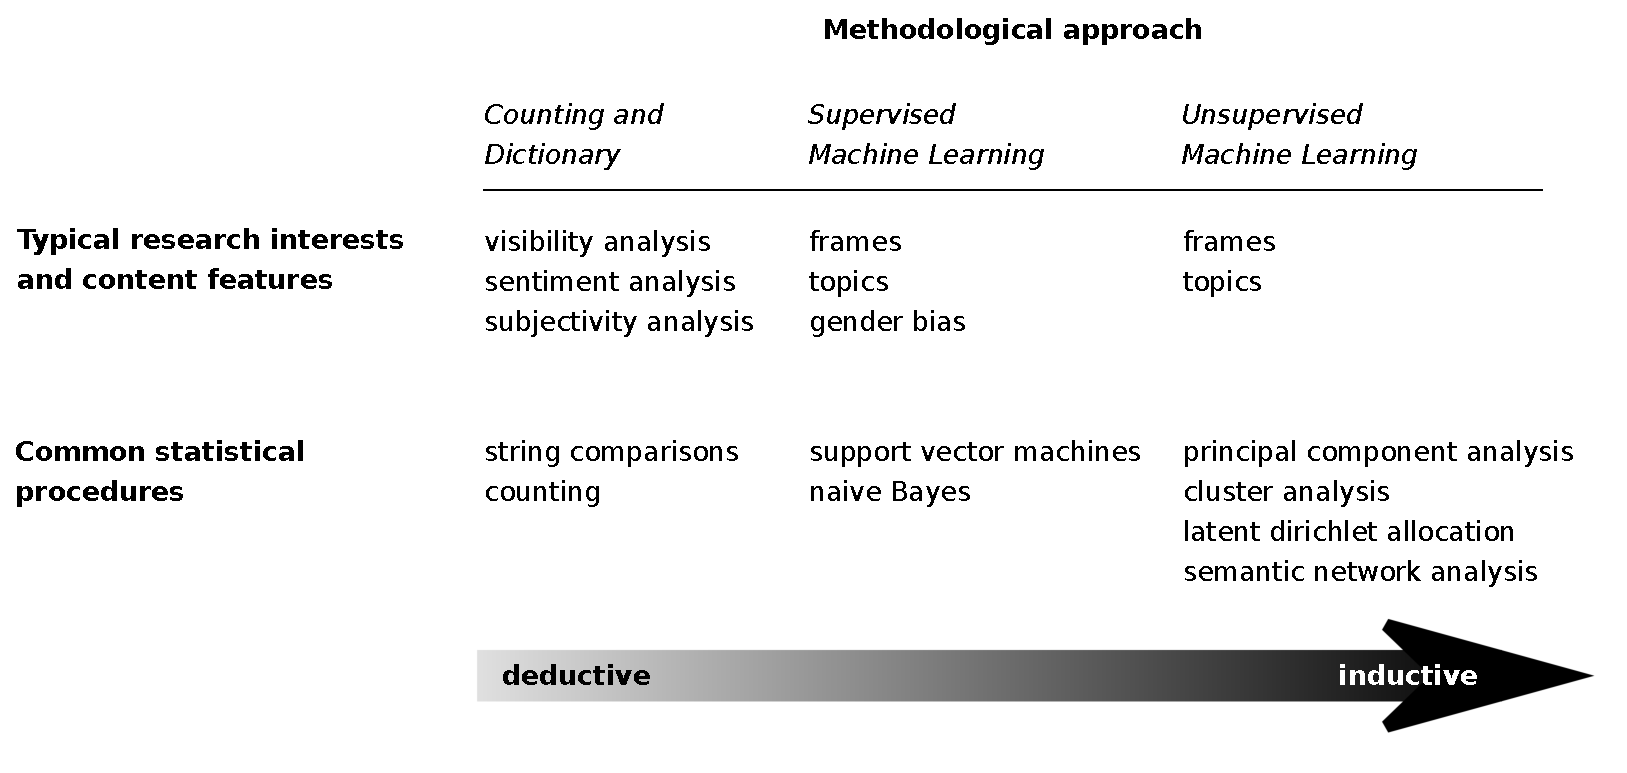
\includegraphics[width=1.0\linewidth]{boumanstrilling2016}
		\label{fig:boumanstrilling2016}
	\end{figure}
	\tiny{Boumans, J. W., \& Trilling, D. (2016). Taking stock of the toolkit: An overview of relevant autmated content analysis approaches and techniques for digital journalism scholars. \emph{Digital Journalism, 4}(1), 8–23. doi:10.1080/21670811.2015.1096598}
\end{frame}




\begin{frame}{Supervised vs. unsupervised learning}
	\begin{columns}[t]
		
		\column{.5\textwidth}
		
		\begin{block}{Unsupervised}<1->
			\begin{itemize}
				\item No manually coded data
				\item We want to identify patterns or to make groups of most similar cases
				%\item Per case, we want to know to which group it belongs
			\end{itemize}
		\end{block}
		{\footnotesize{
				\onslide<2->{Example: We have a dataset of Facebook-massages on an organizations' page. We use clustering to group them and later interpret these clusters (e.g., as complaints, questions, praise, \ldots)}
			}}
			
			\column{.5\textwidth}
			\begin{block}{Supervised}<3->
				\begin{itemize}
					\item We code a small dataset by hand and use it to ``train'' a machine
					\item The machine codes the rest 
				\end{itemize}
			\end{block}
			
			{\footnotesize{
					\onslide<4->{Example: %We use a hand-coded CSV table with two columns (tweet and gender of the sender) as training dataset and then predict for a different dataset per tweet if it was sent by a man or a woman.
						We have 2,000 of these messages grouped into such categories by human coders. We then use this data to group all remaining messages as well.
					}
				}}
				
			\end{columns}
		\end{frame}
		
		



\begin{frame}[plain]
	inductive and bottom-up:\\ \textbf{unsupervised machine learning}\\
	\vspace{1cm}\hspace{1cm} \onslide<2> \footnotesize{(something you aready did in your Bachelor -- no kidding.)}
\end{frame}



\subsection{PCA}




\begin{frame}{Principal Component Analysis? How does \emph{that} fit in here?}
	\onslide<2>{In fact, PCA is used everywhere, even in image compression}
	
	\begin{block}<3->{PCA in ACA}
		\begin{itemize}
			\item Find out what word cooccur (inductive frame analysis)
			\item Basically, transform each document in a vector of word frequencies and do a PCA
		\end{itemize}
	\end{block}
	%\onslide<4>{\textbf{But we'll look at the state of the art instead: Latent Dirichlet Allication (LDA)}}
\end{frame}

\begin{frame}[fragile]{A so-called term-document-matrix}
\begin{lstlisting}
      w1,w2,w3,w4,w5,w6 ...
text1, 2, 0, 0, 1, 2, 3 ...
text2, 0, 0, 1, 2, 3, 4 ...
text3, 9, 0, 1, 1, 0, 0 ...
...
\end{lstlisting}
\vspace{1cm}
\onslide<2>{These can be simple counts, but also more advanced metrics, like tf-idf scores (where you weigh the frequency by the number of documents in which it occurs), cosine distances, etc.}
\end{frame}


\begin{frame}{PCA: implications and problems}
	\begin{itemize}
		\item given a term-document matrix, easy to do with any tool
		\item probably extremely skewed distributions
		\item some problematic assumptions: does the goal of PCA, to find a solution in which one word loads on \emph{one} component match real life, where a word can belong to several topics or frames?
	\end{itemize}
\end{frame}





\subsection{LDA}


\begin{frame}{}
	Enter \textbf{topic modeling with Latent Dirichlet Allocation (LDA)}
\end{frame}








\begin{frame}{LDA, what's that?}
	\begin{block}{No mathematical details here, but the general idea}
		\begin{itemize}
			\item There are $k$ topics, $T_1$\ldots$T_k$
			\item Each document $D_i$ consists of a mixture of these topics, e.g.$80\% T_1, 15\% T_2, 0\% T_3, \ldots 5\% T_k $
			\item On the next level, each topic consists of a specific probability distribution of words
			\item Thus, based on the frequencies of words in $D_i$, one can infer its distribution of topics
			\item Note that LDA (like PCA) is a Bag-of-Words (BOW) approach
		\end{itemize}
	\end{block}
	
\end{frame}




\begin{frame}[fragile]{Doing a LDA in Python}
You can use gensim ({\v R}eh{\r u}{\v r}ek \& Sojka, 2010) for this.
%
%Let us assume you have a list of lists of words (!) called \texttt{texts}:
%
%\begin{lstlisting}
%articles=['The tax deficit is higher than expected. This said xxx ...', 'Germany won the World Cup. After a']
%texts=[art.split() for art in articles]
%\end{lstlisting}
%which looks like this:
%\begin{lstlisting}
%[['The', 'tax', 'deficit', 'is', 'higher', 'than', 'expected.', 'This', 'said', 'xxx', '...'], ['Germany', 'won', 'the', 'World', 'Cup.', 'After', 'a']]
%\end{lstlisting}

\tiny{{\v R}eh{\r u}{\v r}ek, R., \& Sojka, P. (2010). Software framework for topic modelling with large corpora. \emph{Proceedings of the LREC 2010 Workshop on New Challenges for NLP Frameworks}, pp. 45–50. Valletta, Malta: ELRA. }
	
\end{frame}




\begin{frame}[plain,fragile]
\begin{lstlisting}
from gensim import corpora, models

NTOPICS = 100
LDAOUTPUTFILE="topicscores.tsv"

# Create a BOW represenation of the texts
id2word = corpora.Dictionary(texts)
mm =[id2word.doc2bow(text) for text in texts]

# Train the LDA models.
lda = models.ldamodel.LdaModel(corpus=mm, id2word=id2word, num_topics=NTOPICS)

# Print the topics.
for top in lda.print_topics(num_topics=NTOPICS, num_words=5):
    print ("\n",top)

# save topic scores
scoresperdoc=lda.inference(mm)
with open(LDAOUTPUTFILE,"w",encoding="utf-8") as fo:
  for row in scoresperdoc[0]:
    fo.write("\t".join(["{:0.3f}".format(score) for score in row]))
    fo.write("\n")
\end{lstlisting}

\end{frame}




\begin{frame}[fragile]{Output: Topics (below) \& topic scores (next slide)}
\begin{lstlisting}
0.069*fusie + 0.058*brussel + 0.045*europesecommissie + 0.036*europese + 0.023*overname
0.109*bank + 0.066*britse + 0.041*regering + 0.035*financien + 0.033*minister
0.114*nederlandse + 0.106*nederland + 0.070*bedrijven + 0.042*rusland + 0.038*russische
0.093*nederlandsespoorwegen + 0.074*den + 0.036*jaar + 0.029*onderzoek + 0.027*raad
0.099*banen + 0.045*jaar + 0.045*productie + 0.036*ton + 0.029*aantal
0.041*grote + 0.038*bedrijven + 0.027*ondernemers + 0.023*goed + 0.015*jaar
0.108*werknemers + 0.037*jongeren + 0.035*werkgevers + 0.029*jaar + 0.025*werk
0.171*bank + 0.122* + 0.041*klanten + 0.035*verzekeraar + 0.028*euro
0.162*banken + 0.055*bank + 0.039*centrale + 0.027*leningen + 0.024*financiele
0.052*post + 0.042*media + 0.038*nieuwe + 0.034*netwerk + 0.025*personeel
...
\end{lstlisting}
\end{frame}


\begin{frame}[plain]
	\makebox[\linewidth]{
		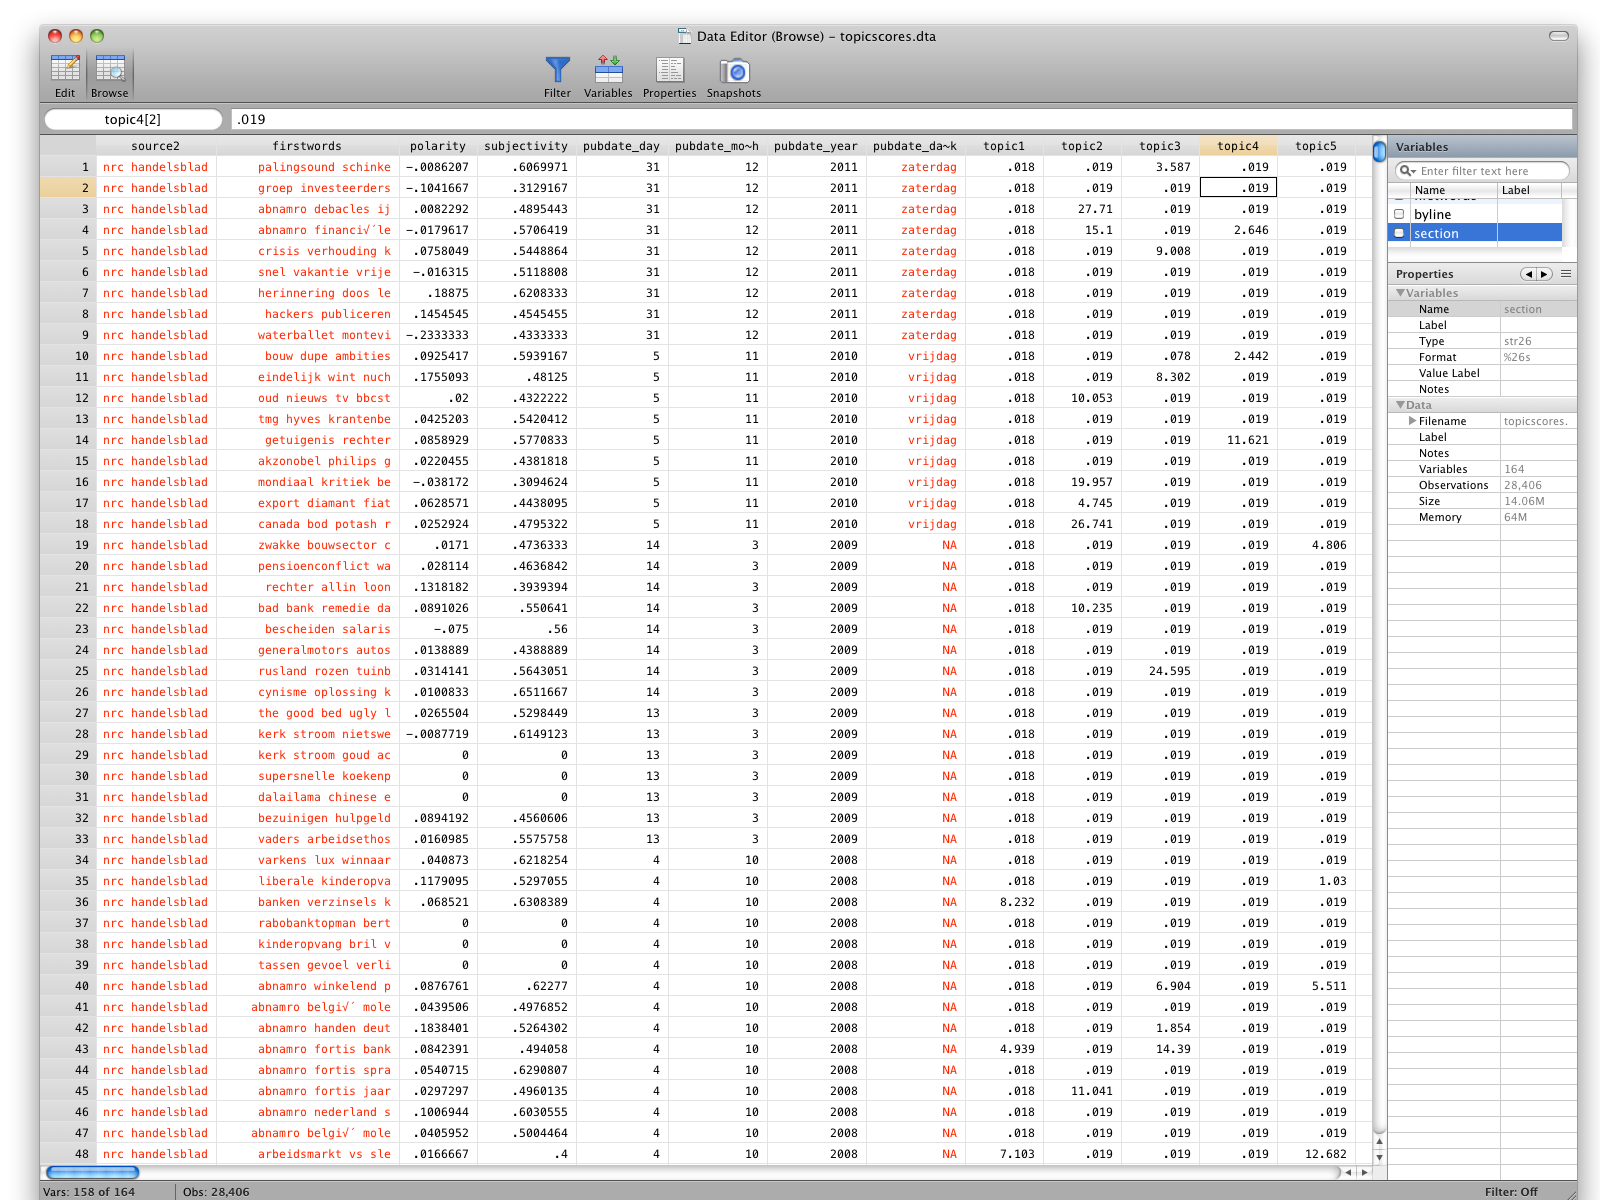
\includegraphics[width=\paperwidth,height=\paperheight,keepaspectratio]{topicscores}}
\end{frame}




\begin{frame}[fragile]{Visualization with pyldavis}
\begin{lstlisting}
import pyLDAvis
import pyLDAvis.gensim
% first estiate gensim model, then:
vis_data = pyLDAvis.gensim.prepare(lda,mm,id2word)
pyLDAvis.display(vis_data)
\end{lstlisting}
\makebox[\linewidth]{
	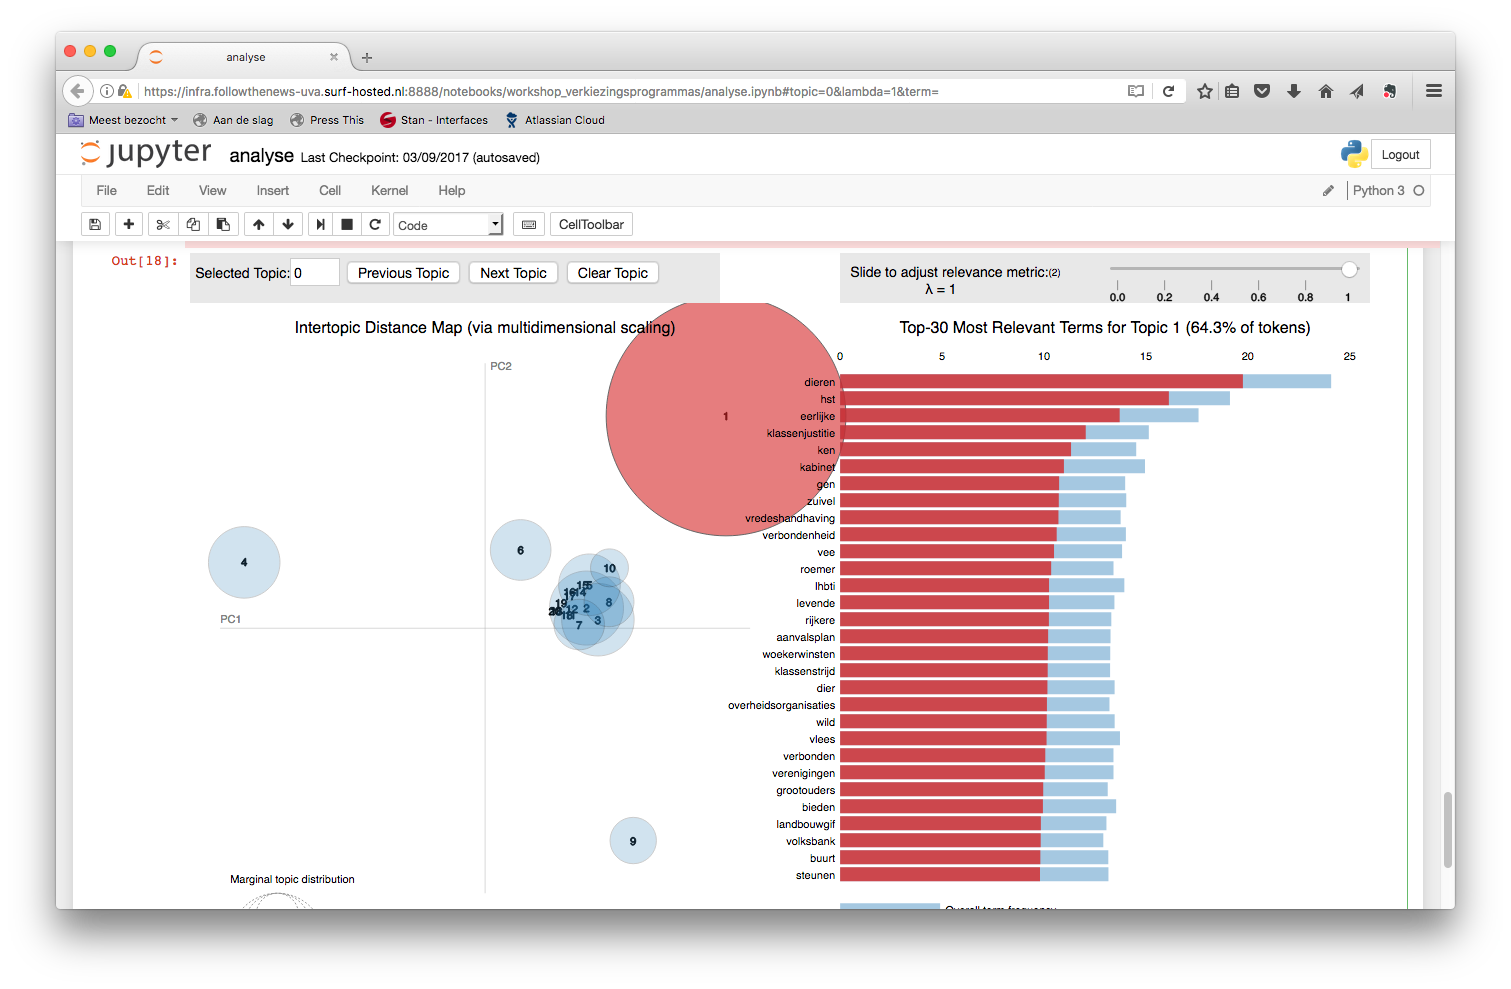
\includegraphics[width=\paperwidth,height=.5\paperheight,keepaspectratio]{pyldavis}}
\end{frame}





\section*{Supervised Machine Learning}

\begin{frame}[plain]
	\textbf{Supervised machine learning} is something for another time \ldots
\end{frame}



\section{Example and exercise}
\begin{frame}{Example and exercise}
Let's have a look at the EU-speech dataset (Jupyter Notebook). I'll first walk you through the example, afterwards, you have time to play with the data yourself.
\end{frame}

\begin{frame}[plain]
	\huge
	\centering
	Damian Trilling\\ \vspace{0.5cm}
	d.c.trilling@uva.nl\\
	@damian0604\\
	www.damiantrilling.net\\
\end{frame}




\end{document}


